\documentclass[a4paper,11pt]{article}

\usepackage[utf8]{inputenc} % Unicode support (Umlauts etc.)
\usepackage[ngerman]{babel} % Change hyphenation rules
\usepackage{ziffer} % , können in Zahlen verwendet werden ohne Formatierung kaputt zu machen
\usepackage[top=30mm,right=20mm,bottom=15mm,left=25mm,includefoot,headheight=32pt]{geometry} % Seitenränder

\usepackage{lmodern,textcomp,amsfonts} % The package supports the Text Companion fonts, which provide many text symbols
\usepackage[fleqn]{amsmath} % Formatierte Gleichungen
\usepackage{graphicx} % Grafiken
\usepackage{xcolor} % Farbe in Text
\usepackage{fancyhdr} % Seitenstil mit Kopfzeile etc.
\usepackage{cases} % Fallunterscheidungen mathematisch übereinander

\usepackage{fontawesome}

\usepackage{tikz} % Graphen
\usetikzlibrary{positioning}

\usepackage{tcolorbox}

\newtcbox{\wbox}{left=0pt, right=0pt, top=0pt, bottom=0pt, arc=0pt, boxrule=0pt, colback=white, colframe=white}

\pagestyle{fancy}
\fancyhf{}
\lhead{
    Lösung \\
    Übungsblatt 1
}
\rhead{Gruppe 3 \\Nils \textbf{Hodys}, Sascha \textbf{Majewsky}}
\rfoot{Seite \thepage}

\setlength{\parindent}{0cm} % Keine Einrückung der 1. Zeile eines Absatzes

\begin{document}

\raggedright % Alles Linksbündig
\setlength{\mathindent}{0cm} % align* nicht eingerückt

\section*{Aufgabe 1}

\textbf{1)} nicht linear aufgrund von Multiplikation in 2. Restriktion \\
\textbf{2)} linear \\
\textbf{3)} linear, jedoch fehlt die Nichtnegativitätsbedingung \\
\textbf{4)} nicht linear aufgrund des Exponenten in der 1. Restriktion \\

\section*{Aufgabe 2}
Begründungen graphisch. Restriktionen sind durch farbige Flächen dargestellt. \\

\subsection*{1)}
Modell hat keine zulässige Lösung. Es gibt keinen nicht-negativen Bereich, in dem alle Restriktion erfüllt sind. Das einzeichnen einer Iso-Gewinngerade ist an keiner Stelle sinnvoll. \newline

\begin{centering}
	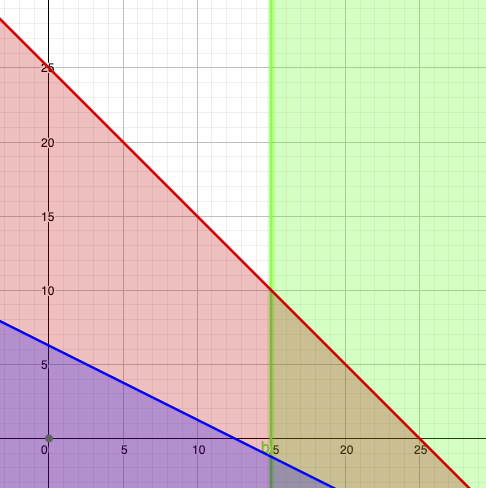
\includegraphics[width=.7\linewidth]{src/a2_1.png}
\end{centering}

\subsection*{2)}
Die Lösung ist mehrdeutig. Die schwarz gezeichnete Iso-Gewinngerade liegt auf der Grenze der 1. Restriktion (Rot). Mögliche Lösungen sind überall entlang der Iso-Gewinngeraden innerhalb der Restriktionen. \newline

\begin{centering}
	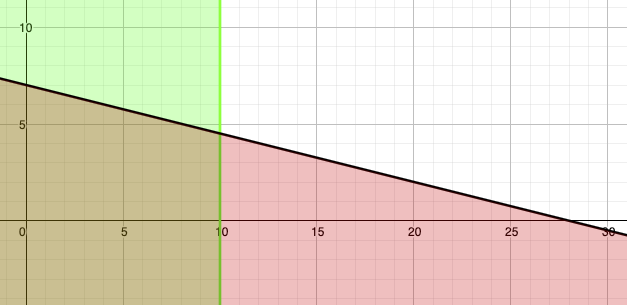
\includegraphics[width=.7\linewidth]{src/a2_2.png}
\end{centering}

\subsection*{3)}
Der Lösungsraum ist offen. Eine Lösung kann nicht bestimmt werden, die Iso-Gewinngerade kann beliebig im Lösungsraum platziert werden. \newline

\begin{centering}
	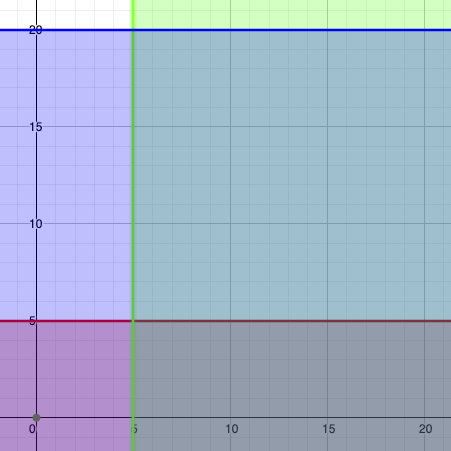
\includegraphics[width=.7\linewidth]{src/a2_3.png}
\end{centering}

\subsection*{4)}
Die Lösung befindet sich am Schnittpunkt der Iso-Gewinngerade (schwarz) mit den Restriktionen. \newline

\begin{centering}
	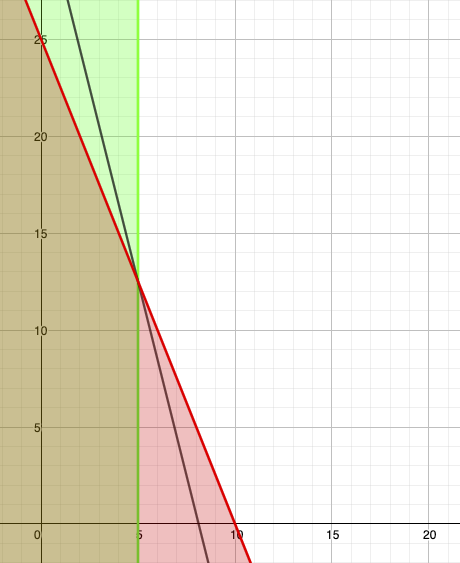
\includegraphics[width=.7\linewidth]{src/a2_4.png}
\end{centering}

\section*{Aufgabe 3}

\subsection*{Entscheidungsvariablen}
$x_H$ : Holzmenge in 0,5kg-Einheiten pro Tag \\
$x_B$ : Bioabfallmenge in 0,5kg-Einheiten pro Tag \\

\subsection*{Zielfunktion}
Die Zielfunktion $z$ ist in EUR Umsatz pro Tag angegeben uns soll maximiert werden. \\

\subsection*{Modell}
\begin{align*}
    \text{max. } & z = 30x_H + 20x_B && \\
    \text{s.t. } & x_H + x_B \le 1300 && \text{Maschinenkapazität 650kg / 1300 BTPs} \\
    & x_H \le 980 && \text{Holzmenge begrenzt auf 490kg/Tag} \\
    & x_B \ge 580 && \text{Es müssen 290kg Bioabfall pro Tag verarbeitet werden} \\
    & x_H, x_B \ge 0 && \text{NBB} \\
\end{align*}

Lösung laut Solver: \\
$x_H = 720$ \\
$x_B = 580$ \\
~\newline
Es werden täglich 720 BTPs aus Holz und 580 BTPs aus Bioabfall hergestellt. Damit wird ein Umsatz von 33.200€ erzielt.

\end{document}